\section{Experimental details}\label{sec:exp_details}

% \lc{Should be put into appendix later.}

This section provides implementation details of our experiments and some additional simulations.
% Our code is available at \url{https://anonymous.4open.science/r/in-context-rl}.

\subsection{Implementation details}
\paragraph{Model and embedding}

Our experiments use a GPT-2 model \citep{radford2019language} with ReLU activation layers. The model has $L=8$ attention layers, $M=4$ attention heads, and embedding dimension $D=32$. Following standard implementations in~\cite{vaswani2017attention}, we add Layer Normalization~\citep{ba2016layer} after each attention and MLP layer to facilitate optimization. We consider the embedding and extraction mappings as described in Appendix~\ref{sec:tf_embed_bandit}, and train transformer $\TF_{\EstPar}(\cdot)$ via  maximizing Eq.~\eqref{eq:general_mle}.
\paragraph{Online algorithms}
We compare the regret of the algorithm induced by the transformer with empirical average, Thompson sampling, and LinUCB (or UCB for Bernoulli bandits).
\begin{itemize}
\item[\textbf{(Emp)}]\textbf{Empirical average}. 
For time $t\leq A$, the agent selects each action once. For time $t>A$, the agent computes the average of the historical rewards for each action and selects the action with the maximal
averaged historical rewards.
\item[\textbf{(TS)}]\textbf{Thompson sampling}. For linear bandits with Gaussian noises, we consider Thompson sampling introduced in Appendix~\ref{app:ts_algorithm_formula} with $\Tpsparn=\sigma=1.5$ and $\lambda=1$ (note that in this case TS does not correspond to posterior sampling as we assume $\bw^*$ follows the uniform distribution on $[0,1]^d$). For Bernoulli bandits,  we consider the standard TS sampling procedure (see, for example, Algorithm 3.2 in~\cite{russo2018tutorial}). 
\item[\textbf{(LinUCB)}]\textbf{Linear UCB and UCB}. For linear bandits, we use LinUCB (Appendix \ref{sec:soft-LinUCB}) with $\lambda=1$ and $\alpha=2$. For multi-armed Bernoulli bandits, LinUCB reduces to UCB, which selects $\action_t=\argmax_{\action\in\actionsp}\{\hat \mu_{t,\action}+\sqrt{1/\Numvi_t(\action)}\}$, where $\mu_{t,\action}$ is the average reward for action $\action$ up to time $t$, and $\Numvi_t(\action)$ is the number of times action $\action$ was selected up to time $t$.
\end{itemize} 
\subsection{Additional experiments and plots}
We provide additional experiments and plots in this section. In all experiments, we choose the number of samples $\Numobs=100$K. 


Additional plots of suboptimality $\<\action_t^*-\action_t,\bw^*\>$ over time are shown in Figure~\ref{fig:subopt_1} for the two experiments in Section~\ref{sec:experiments}. In both cases, the transformer is able to imitate the expected expert policy $\osAlg_{\shortexp}$, as its suboptimality closely matches   $\osAlg_{\shortexp}$ (LinUCB and TS for the left and right panel, respectively).  While the empirical average (Emp) has lower suboptimality early on, its gap does not converge to zero. In contrast, both LinUCB and Thompson sampling are near-optimal up to $\tcO(1)$ factors in terms of their (long-term) regret.\lc{Is this correct?} 

\begin{figure}[ht]
\centering  % Center the figure
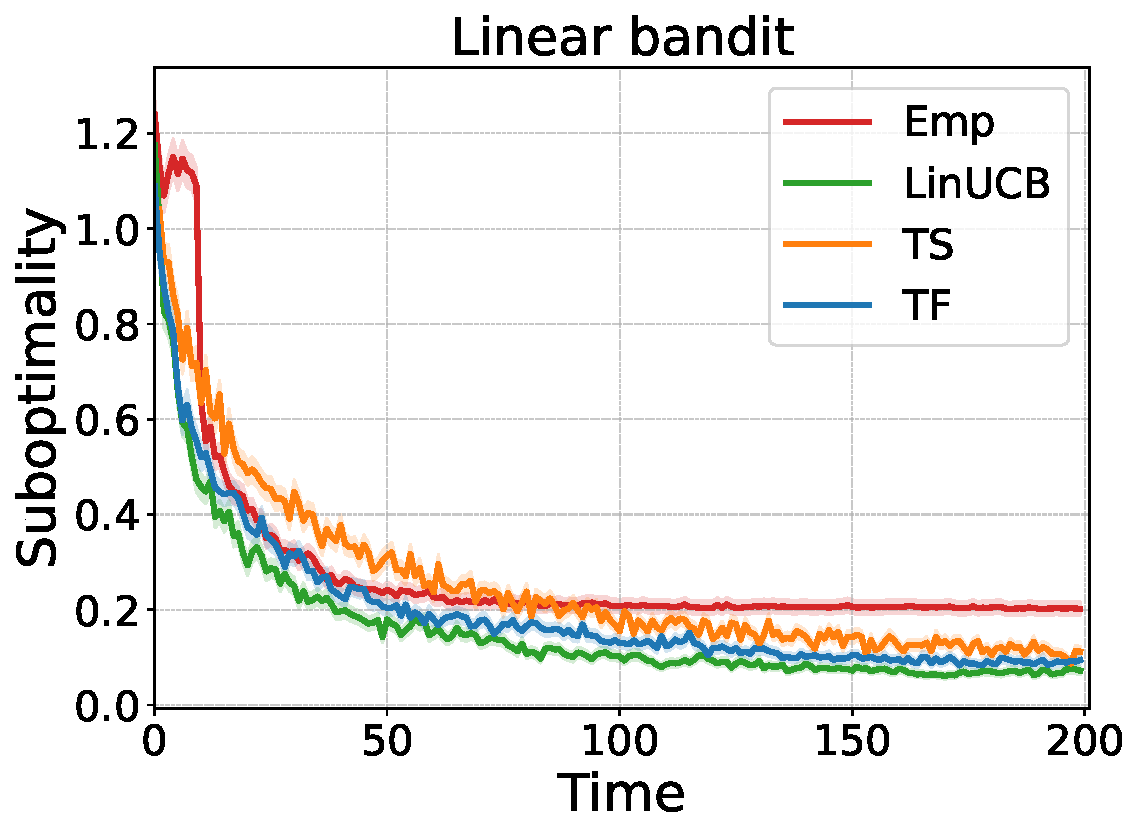
\includegraphics[width=0.46\linewidth]{Sections/figs/record_2_cum_False.pdf}
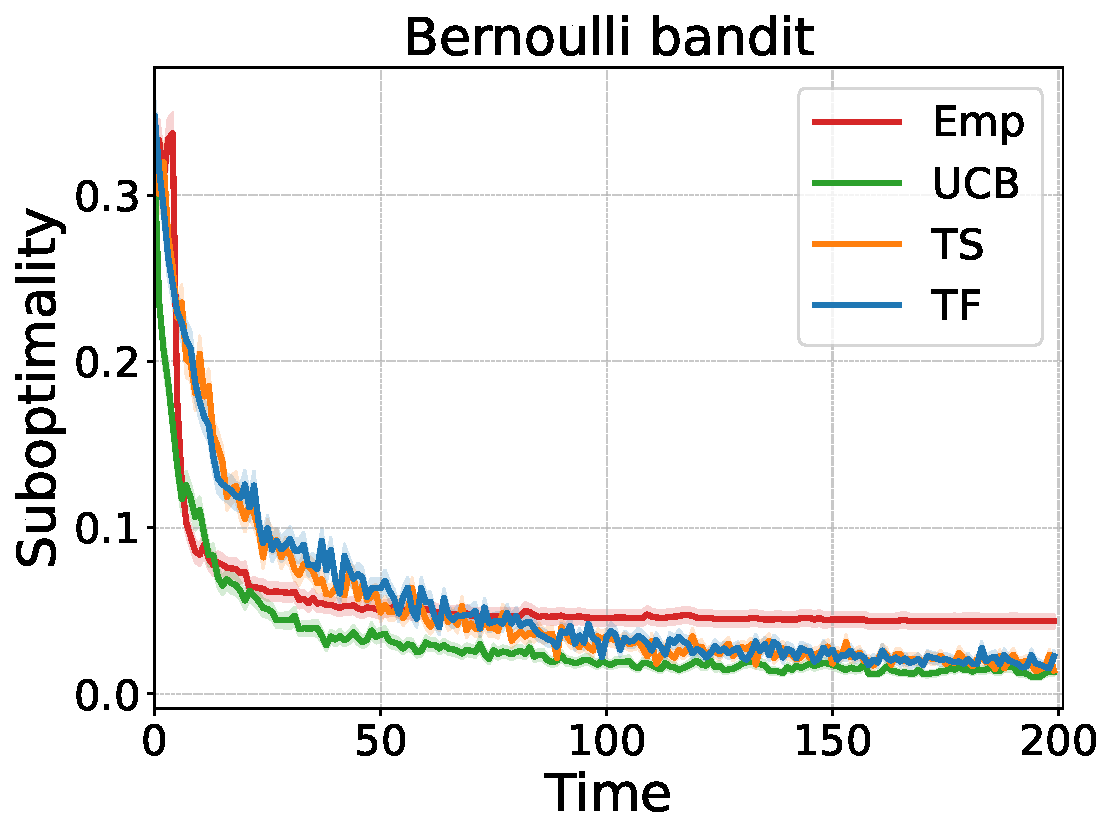
\includegraphics[width=0.45\linewidth]{Sections/figs/record_1_cum_False.pdf}
\caption{Suboptimalities of transformer (TF), empirical average (Emp), Thompson sampling (TS), and LinUCB (or UCB). Left: linear bandit with $d=5$, $A=10$, $\sigma=1.5$, $\sAlg_0=\sAlg_\shortexp=\LinUCB$. Right: Bernoulli bandit with $d=5$, $\sAlg_0=(\sAlg_{\mathrm{unif}}+\sAlg_{\TS})/2$, and $\sAlg_\shortexp=\action_t^*$. The simulation is repeated 500 times. Shading displays the standard deviation of the sub-optimality estimates. %\sm{Check the shades}
} 
\label{fig:subopt_1} 
\end{figure}


Additional simulations were run with $\sAlg_0=\sAlg_{\shortexp}=\UCB$ for Bernoulli bandits, which has fewer actions ($\Numact=5$) than linear bandits ($\Numact=10$). Figure~\ref{fig:linucb_bernoulli} shows the regret and suboptimality of UCB and the transformer overlap perfectly, with both algorithms exhibiting optimal behavior. This suggests the minor gaps between LinUCB and transformer in the left panel of Figure~\ref{fig:regret_1} and \ref{fig:subopt_1} are likely due to limited model capacity. %, compared with the complexity of the bandit problem.

\begin{figure}[ht]
\centering  % Center the figure
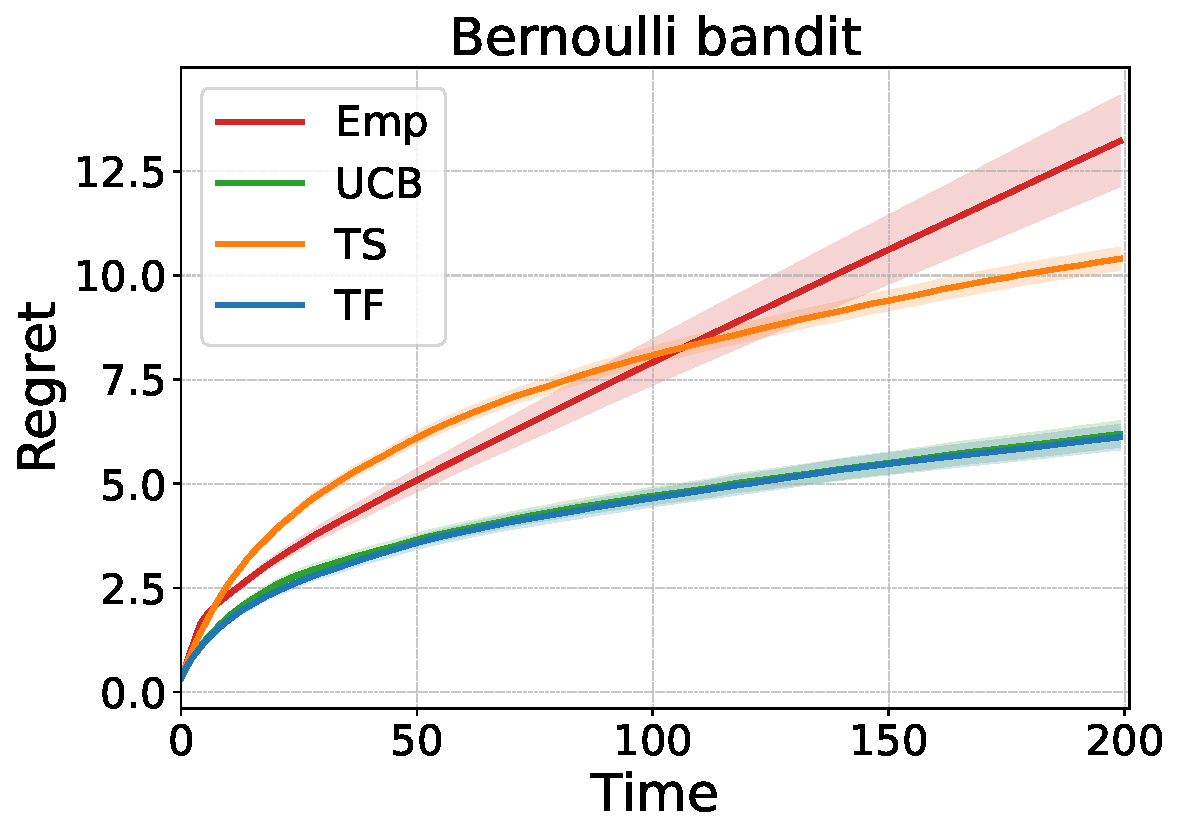
\includegraphics[width=0.47\linewidth]{Sections/figs/record_3_cum_True.pdf}
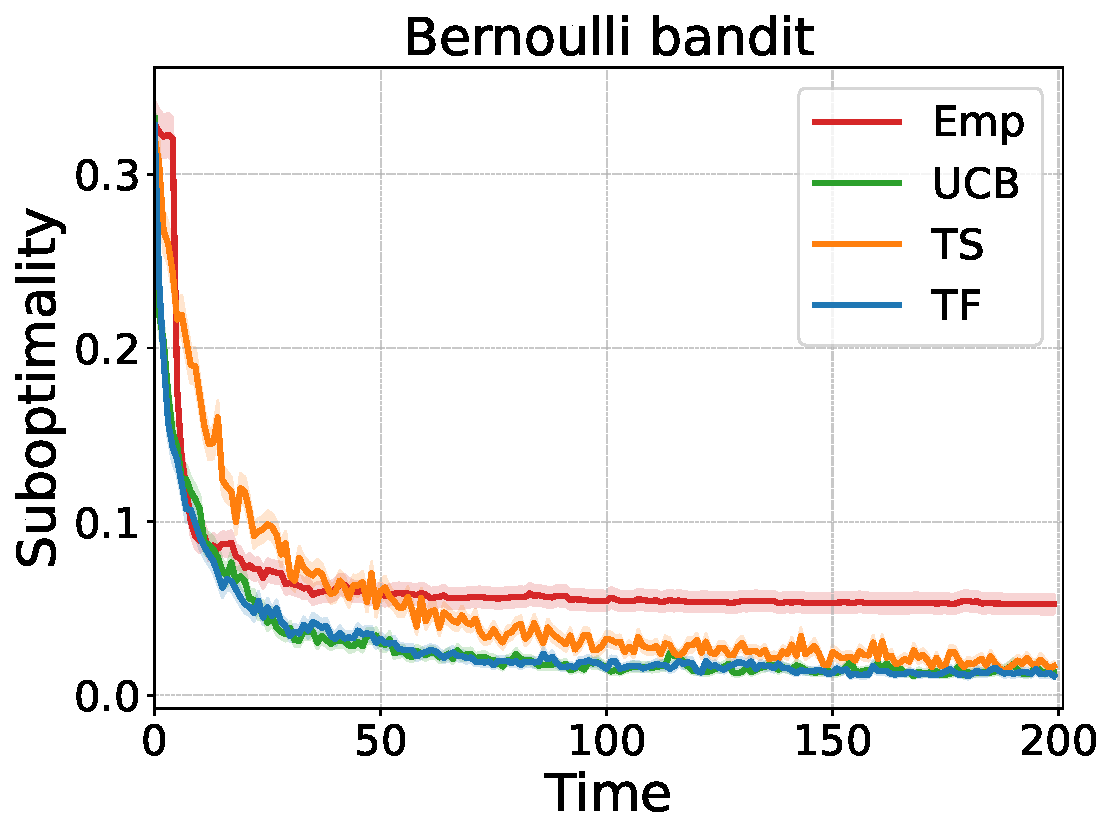
\includegraphics[width=0.45\linewidth]{Sections/figs/record_3_cum_False.pdf}
\caption{Regrets and suboptimalities of transformer (TF), empirical average (Emp), Thompson sampling (TS), and  UCB. Settings: Bernoulli bandit with $d=5$, and $\sAlg_0=\sAlg_\shortexp=\LinUCB$. 
The simulation is repeated 500 times. Shading displays the standard deviation of the estimates. } 
\label{fig:linucb_bernoulli} 
\end{figure}

\subsection{The effect of distribution ratio}

We evaluate the effect of the distribution ratio $\distratio=\distratio_{\osAlg_{\shortexp},\sAlg_0}$ (Definition \ref{def:dist_ratio}) on transformer performance. We consider the Bernoulli bandit setting from Section~\ref{sec:experiments} with expert $\sAlg_\shortexp=\action^*$ giving optimal actions. The context algorithm is $$\sAlg_0=\alpha\sAlg_{\TS}+(1-\alpha)\sAlg_{\unif},$$
mixing uniform policy $\sAlg_{\unif}$ and Thompson sampling $\sAlg_{\TS}$, for $\alpha\in\{0,0.1,0.5,1\}$. The case $\alpha=0$ corresponds to the context algorithm being the i.i.d. uniform policy, and  $\alpha=1$ corresponds to the context algorithm being Thompson sampling. Note that the distribution ratio $\distratio$ may scale as $\cO((1/\alpha)\wedge \Numact^{\cO(\totlen)})$ in the worst case. 

Figure~\ref{fig:compare_ratio} evaluates the learned transformers against Thompson sampling for varying context algorithms.  The left plot shows cumulative regret for all algorithms. The right plot shows the regret difference between transformers and Thompson sampling. The results indicate that an increased distribution ratio impairs transformer regret, as expected. Moreover, it is observed that the transformer, even with the uniform policy (i.e., $\alpha=0$), is capable of imitating Thompson sampling in the early stages $(\mathrm{Time}\leq 30)$, exceeding theoretical predictions. This suggests the transformer can learn Thompson sampling even when the context algorithm differs significantly from the expert algorithm. 




\begin{figure}[ht]
\centering  % Center the figure
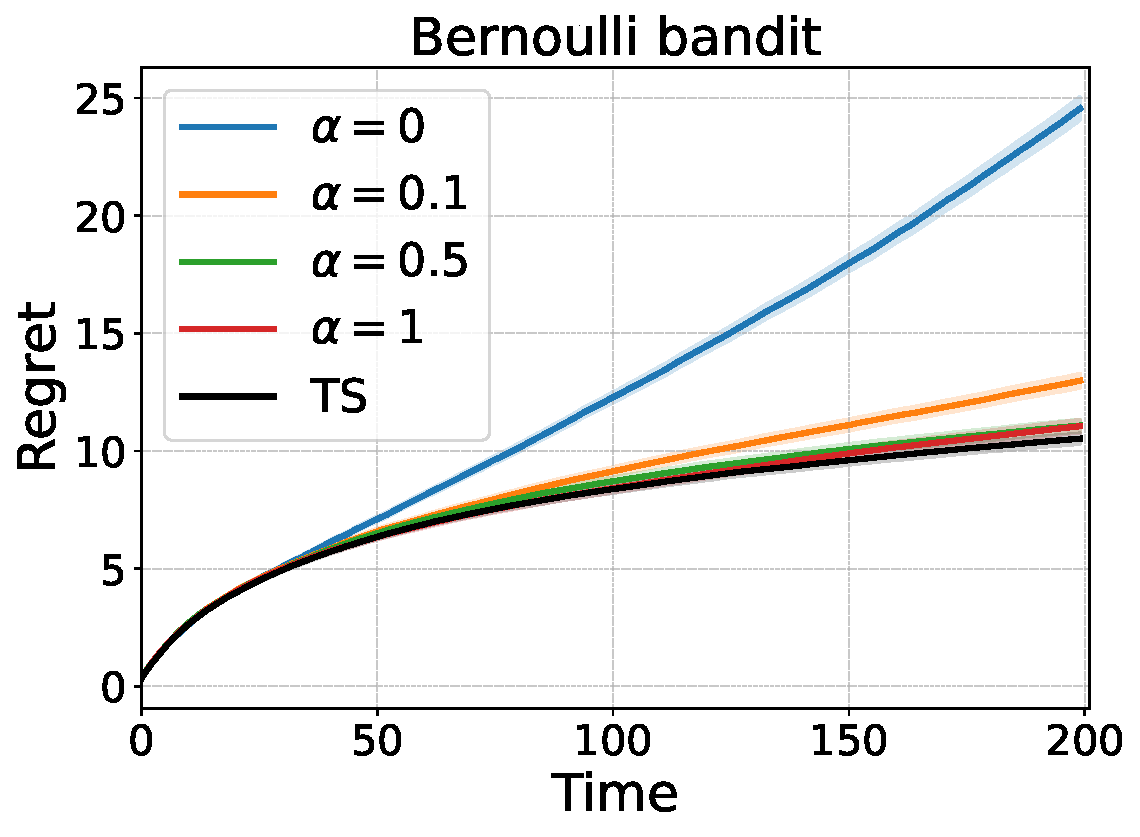
\includegraphics[width=0.45\linewidth]{Sections/figs/record_compare_diff_False.pdf}
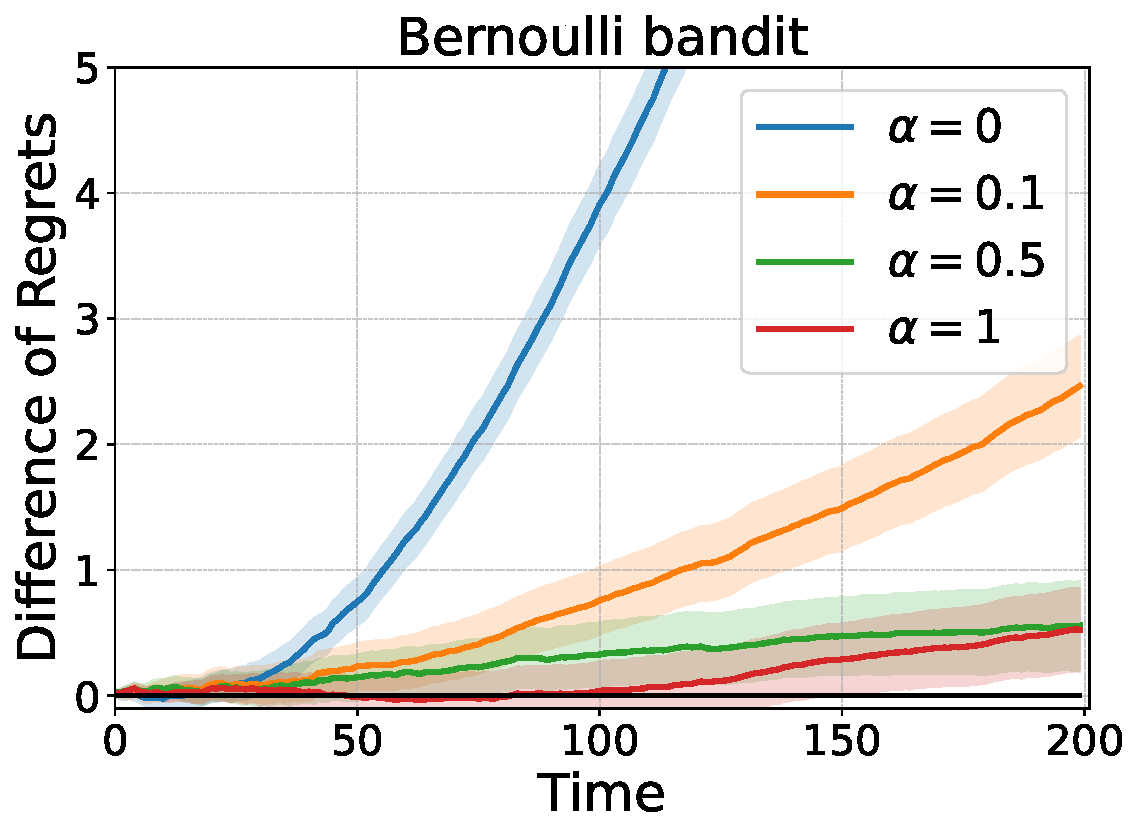
\includegraphics[width=0.45\linewidth]{Sections/figs/record_compare_diff_True.pdf}
\caption{Regrets and difference of regrets between transformers and Thompson sampling, for different context algorithms. Settings: Bernoulli bandit with $d=5$, $\sAlg_\shortexp=\action_t^*$ and $\sAlg_0=\alpha\sAlg_\TS+(1-\alpha)\sAlg_\unif$ with $\alpha \in \{0,0.1,0.5,1\}$. The simulation is repeated 500 times. Shading displays the standard deviation of the estimates. } 
\label{fig:compare_ratio} 
\end{figure}